\documentclass[a4paper,10pt]{article}
\usepackage{graphicx}
\usepackage{verbatim}
% \usepackage{lstlisting}
\usepackage{subfig}
\usepackage{float}
 \usepackage[spanish]{babel}   %ver bien como es
\usepackage[utf8]{inputenc}


\begin{document}

\tableofcontents

\newpage


\section*{Introducci\'on}
\addcontentsline{toc}{section}{Introducci\'on}
El siguiente trabajo tiene como fin aplicar los conocimientos adquiridos en Organización del Computador II, Dpto de Computación, Facultad de Ciencias Exactas y Naturales, Universidad de Buenos Aires.	El proyecto incluye la creacion de un "Sistema Operativo" programado en el lenguaje C++.



\section*{Organizaci\'on del C\'odigo Fuente}
\addcontentsline{toc}{section}{Organizaci\'on del C\'odigo Fuente}
A continuacion se presenta la jerarquia del codigo fuente.

\begin{figure}[H]
\centering
\subfloat{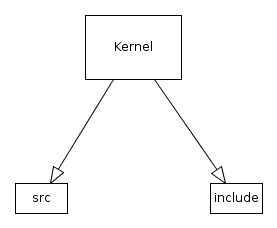
\includegraphics[width=0.8\textwidth]{imagenes/goblal.png}}
\caption{Diagrama de jerarquia de archivos.}
\end{figure}

\begin{figure}[H]
\centering
\subfloat{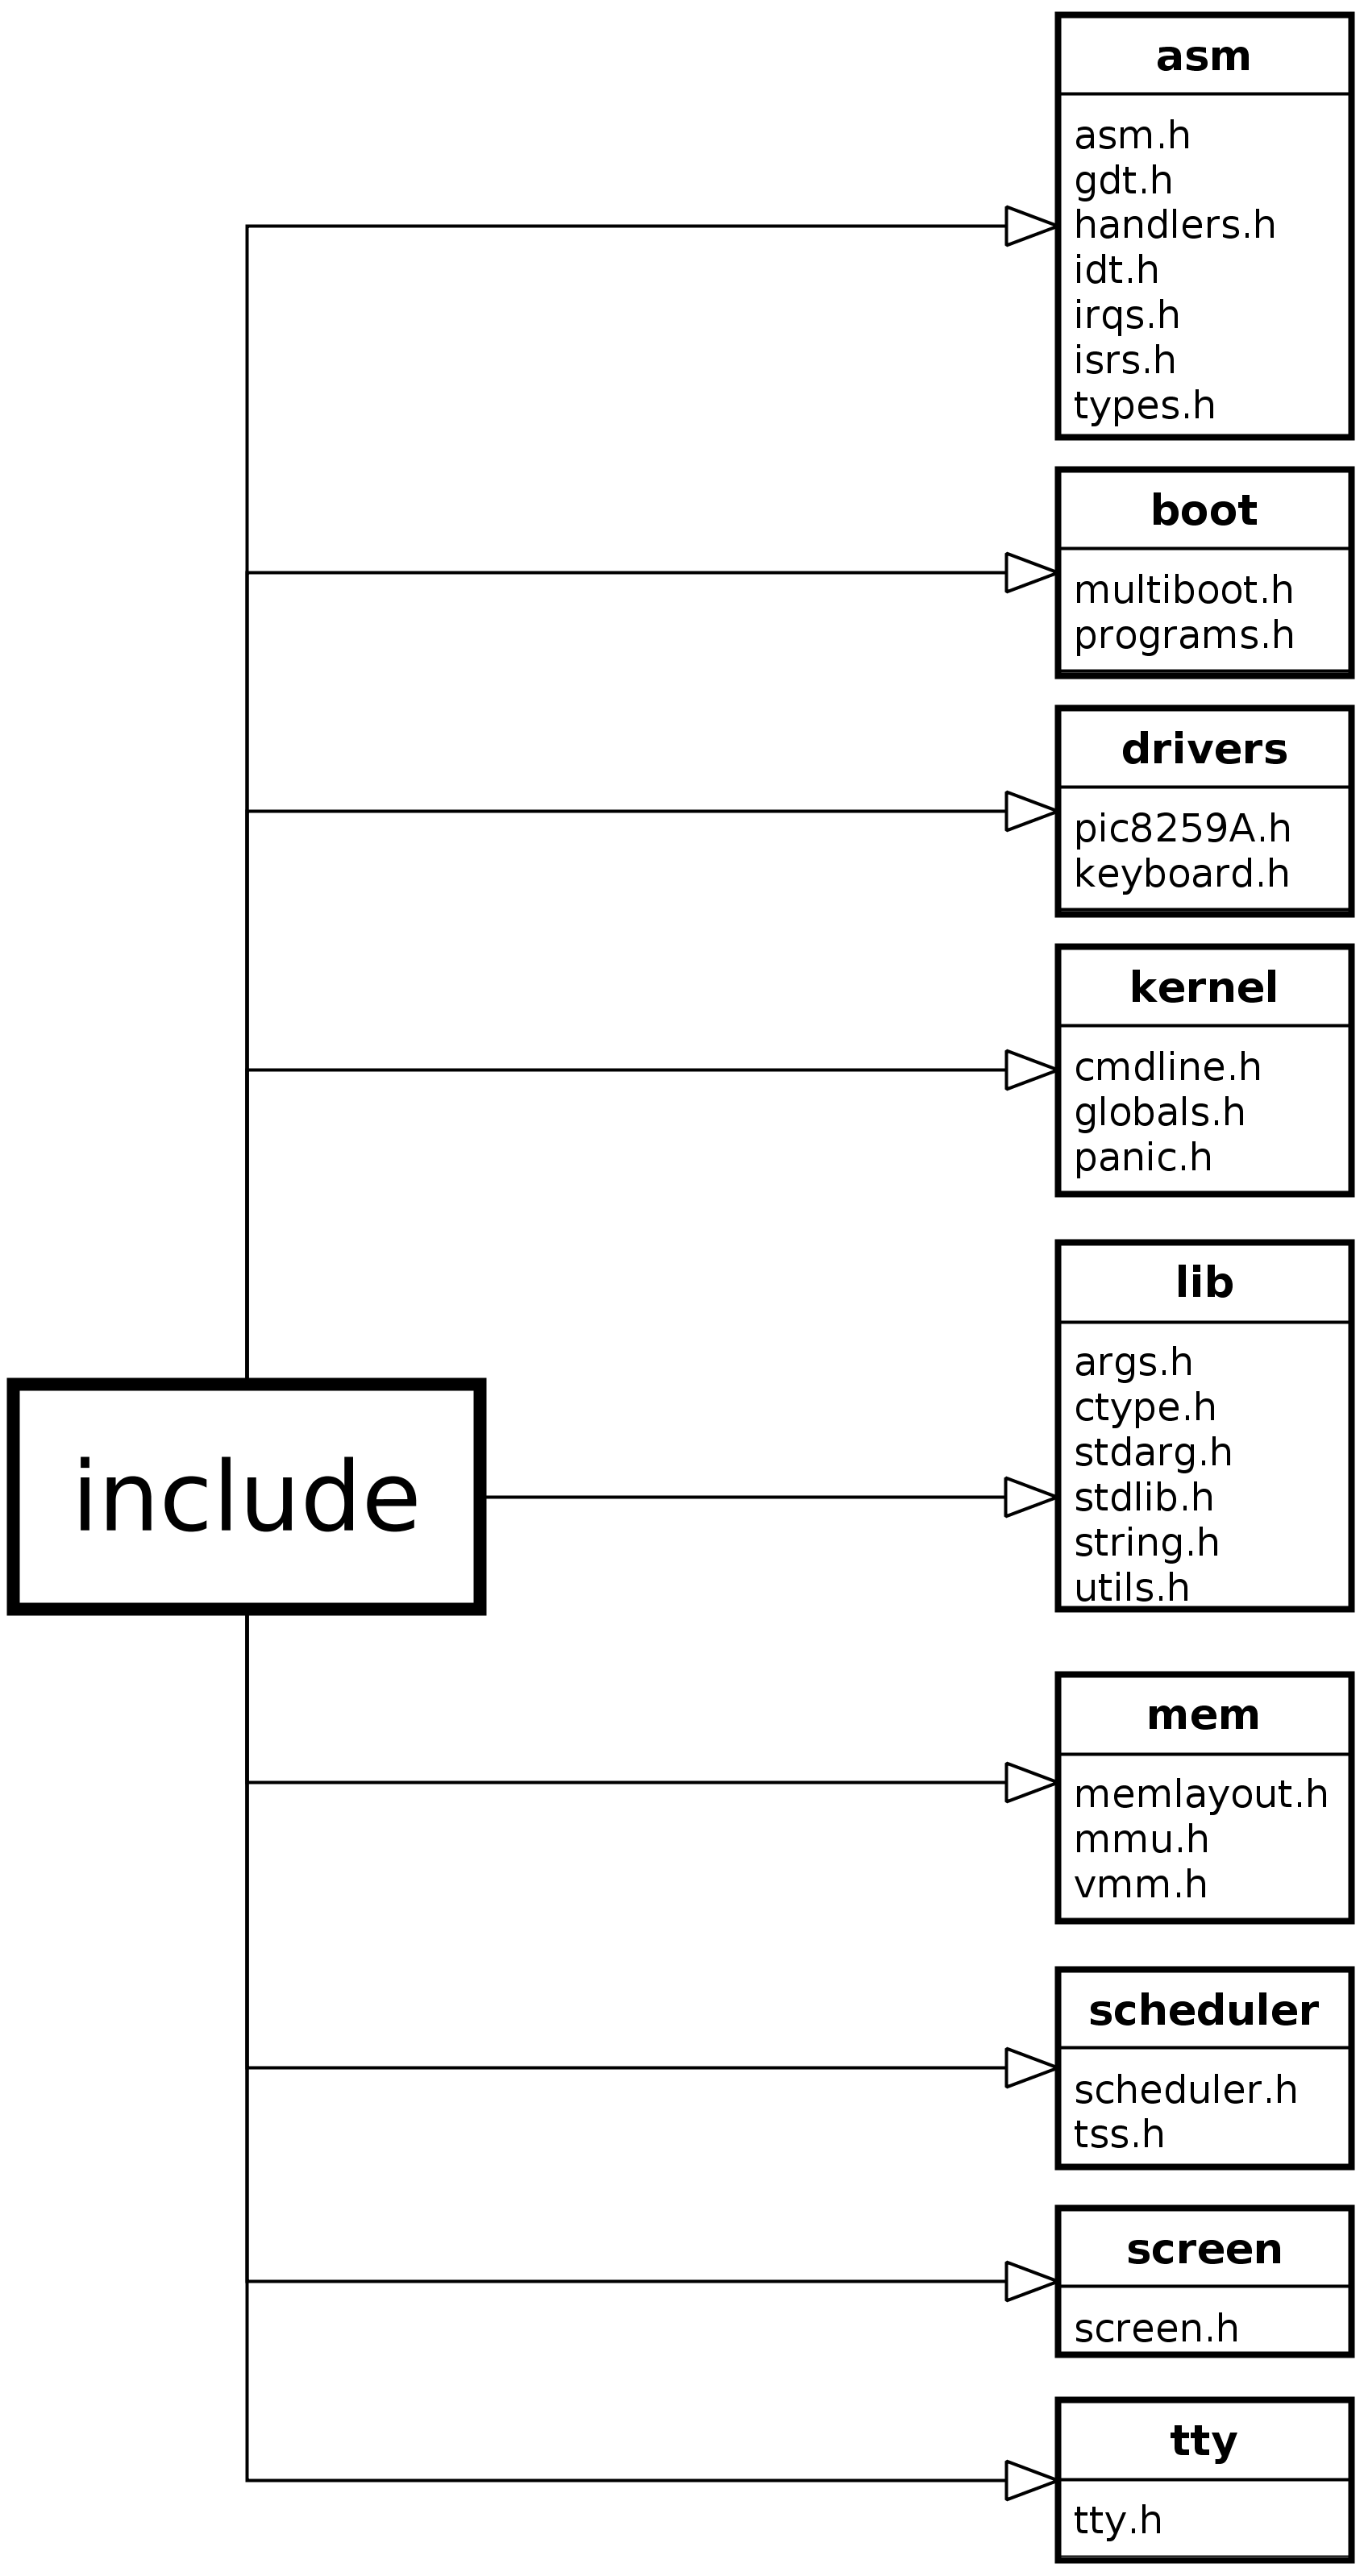
\includegraphics[width=0.8\textwidth]{imagenes/diagrama_de_archivos_include.png}}
\caption{Diagrama de jerarquia de archivos (cont).}
\end{figure}

\begin{figure}[H]
\centering
\subfloat{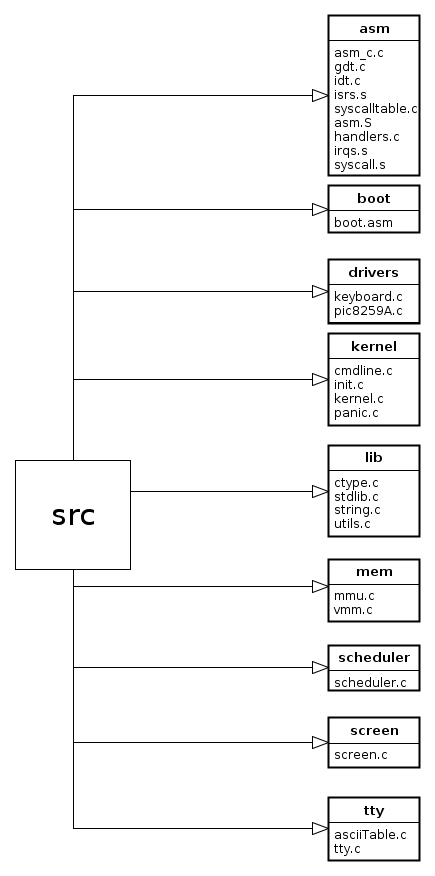
\includegraphics[width=0.8\textwidth]{imagenes/diagrama_de_archivos_src.png}}
\caption{Diagrama de jerarquia de archivos (cont).}
\end{figure}


\section*{Bootloader}
\addcontentsline{toc}{section}{Bootloader}


\section*{Administrador de memoria}
\addcontentsline{toc}{section}{Administrador de memoria}
El administrador de memoria cuenta con la siguientes funciones exportables:

\begin{itemize}
\item \begin{verbatim} void mmu_init(multiboot_info_t  mbd) \end{verbatim} 
\item \begin{verbatim} uint8_t mmu_alloc(uint32_t  pdt, uint32_t  va, uint32_t  pa,
 uint8_t perm) \end{verbatim} 
\item \begin{verbatim} uint8_t mmu_alloc_at_VA( pde_t  pdt, uint32_t va, uint8_t perm,
 uint8_t force_dealloc ) \end{verbatim} 
\item \begin{verbatim} uint8_t mmu_map_pa2va(pde_t  pdt, uint32_t pa, uint32_t va, uint8_t perm,
 uint8_t force_dealloc ) \end{verbatim}    
\item \begin{verbatim} uint8_t mmu_free( pde_t  pdt, uint32_t va ) \end{verbatim} 
\item \begin{verbatim} uint32_t mmu_get_free_frame_count() \end{verbatim} 
\item \begin{verbatim} uint8_t mmu_install_task_pdt(uint32_t  va, uint32_t  pa) \end{verbatim} 
\item \begin{verbatim} uint8_t mmu_uninstall_task_pdt(pde_t  task_pdt) \end{verbatim} 
\item \begin{verbatim} uint8_t mmu_kalloc( uint32_t  va ) \end{verbatim} 
\end{itemize}


\subsection*{ void mmu\_init(multiboot\_info\_t  mbd)}
Inicializa la Memory Management Unit. Para ello utilizando la informacion provista por GRUB inicializa las estructuras de control de memoria y se encarga de llamar a las funciones necesarias para instalar la GDT definitiva y pasar a paginacion mdb Puntero a estructura multiboot\_info\_t provista por GRUB al inicio del kernel mmu\_install\_gdt, mmu\_init\_paging, mmu\_build\_kernel\_heap.

\subsection*{uint8\_t mmu\_alloc(uint32\_t  pdt, uint32\_t  va, uint32\_t  pa, uint8\_t perm)}
  Toma un frame fisico libre de 4kb y lo mapea dentro de la primera direccion virtual disponible para la 
   PDT pasada como parametro con los permisos solicitados. Devuelve ademas la direccion fisica asociada.
  
     pdt Puntero a la pdt sobre la cual se quiere realizar el mapeo \\
     va  Puntero donde se guarda la direccion virtual donde se realizo el mapeo\\
     pa  Puntero donde se guarda la direccion fisica\\
     perm Permisos asignados a la pagina mapeada\\
     Devuelve E\_MMU\_SUCCESS si se pudo realizar el alloc correctamente, o E\_MMU\_NO\_MEMORY en caso de error\\
     mmu\_free, mmu\_alloc\_at\_VA, mmu\_map\_pa2va.

\subsection*{uint8\_t mmu\_alloc\_at\_VA( pde\_t  pdt, uint32\_t va, uint8\_t perm, uint8\_t force\_dealloc )}
   Obtiene un frame libre y lo intenta mapear en la direccion virtual pasada como parametro.
  
     pdt Puntero a la PDT sobre la cual se realiza el mapeo
     va Direccion virtual usada para mapear el frame libre
     perm Permisos asignados a la nueva pagina mapeada
     force\_dealloc Si en la va pasada como parametro ya habia un mapeo previo, entonces lo deshace si force\_dealloc==1
     Devuelve E\_MMU\_SUCCESS si se realizo el mapeo correctamente, E\_MMU\_INVALID\_VA si ya habia un mapeo y force\_dealloc==0 o E\_MMU\_NO\_MEMORY si no se pudo realizar
     mmu\_alloc
     mmu\_map\_pa2va
     mmu\_free
     
\subsection*{uint8\_t mmu\_map\_pa2va(pde\_t  pdt, uint32\_t pa, uint32\_t va, uint8\_t perm, uint8\_t force\_dealloc )}   Intenta asociar la va con la pa pasada como parametro para la pdt solicitada.
  
     pdt Puntero a la PDT sobre la cual se realiza el mapeo
     va Direccion fisica usada para realizar el mapeo
     va Direccion virtual usada para mapear la direccion fisica
     perm Permisos asignados a la nueva pagina mapeada
     force\_dealloc Si en la va pasada como parametro ya habia un mapeo previo, entonces lo deshace si force\_dealloc==1
     Devuelve E\_MMU\_SUCCESS si se realizo el mapeo correctamente, E\_MMU\_INVALID\_VA si ya habia un mapeo y force\_dealloc==0 o E\_MMU\_NO\_MEMORY si no se pudo realizar
     mmu\_alloc
     mmu\_alloc\_at\_VA
     mmu\_free

\subsection*{uint8\_t mmu\_free( pde\_t  pdt, uint32\_t va )}
   Dada una PDT, deshace el mapeo de la va, obtiene el frame correspondiente, decrementa su cantidad de 
   referencias (si son 0 lo apila como libre) y realiza invlpg para limpiar la TLB
  
     pdt Puntero a una PDT
     va  Direccion virtual a liberar. Debe ser multiplo de PAGE\_SIZE
     uint8\_t Devuelve E\_MMU\_SUCCESS si la operacion se realizo con exito, o E\_MMU\_INVALID\_VA si la va no pudo ser desmapeada
     mmu\_alloc
     mmu\_alloc\_at\_VA
     invlpg
   
\subsection*{uint32\_t mmu\_get\_free\_frame\_count()}
Devuelve la cantidad de frames libres en memoria fisica

\subsection*{uint8\_t mmu\_install\_task\_pdt(uint32\_t  va, uint32\_t  pa)}

   Instala una nueva PDT para ser usada por una nueva tarea
  
     va Es un puntero a un uint32\_t que se va a utilizar para guardar la va utilizada para mapear la nueva pdt dentro del contexto del kernel
     pa Es un puntero a un uint32\_t que se va a utililar para guardar la pa utilizada para guardar la nueva pdt
     uint8\_t Devuelve E\_MMU\_SUCCESS si se realizo con exito la instalacion, o E\_MMU\_NO\_MEMORY si no hubo memoria disponible para realizar la operacion  
     mmu\_uninstall\_task\_pdt
     
\subsection*{uint8\_t mmu\_uninstall\_task\_pdt(pde\_t  task\_pdt)}
   Desinstala la PDT de una tarea pasada como parametro, realizando todos los desmapeos correspondientes
   
     task\_pdt Puntero a la PDT de la taerea
     uint8\_t
     mmu\_install\_task\_pdt 
   
\subsection*{uint8\_t mmu\_kalloc( uint32\_t  va )}
   Toma un frame fisico libre de 4kb y devuelve su dirección virtual en el contexto del kernel.
  
     va  Puntero donde se guarda la dirección virtual.
     Devuelve E\_MMU\_SUCCESS si se pudo realizar el alloc correctamente, o E\_MMU\_NO\_MEMORY en caso de error
     mmu\_free
     mmu\_alloc\_at\_VA
     mmu\_map\_pa2va
   
\subsection*{Estructura}
\begin{verbatim}
typedef struct page_frame
{
   struct page_frame  next;   proximo frame de la lista de frames libres
   struct page_frame  prev;   frame anterior de la lista de frames libres
   uint32_t ref_count;    cantidad de referencias externas
} page_frame_t;

page directory table entry
typedef uint32_t pde_t; 
page table entry
typedef uint32_t pte_t;
\end{verbatim}

\section*{Interrupciones}
\addcontentsline{toc}{section}{Interrupciones}


\section*{Scheduler}
\addcontentsline{toc}{section}{Scheduler}

Para la realizaci\'on del Scheduler se implement\'o una pol\'itica de Round Robin. Cada tarea tiene un quantum variable que se gasta cada 1 milisegundo y al terminar este se pasa a la ejecuci\'on de la siguiente tarea.

Toda la funcionalidad del Scheduler se encuentra en tres archivos:
\begin{itemize}
\item	- scheduler.h
\item	- tss.h
\item	- scheduler.c
\end{itemize}

En la cual podemos encontrar la siguiente estructura que define a una tarea.

\begin{verbatim}
      typedef struct {
          char hay_tarea;						
          unsigned int quantum_fijo;			
          unsigned int quantum_actual;		
          char *pantalla;					
          void *va_tss;						
          void *pa_tss;						
      } tarea;
\end{verbatim}

Contamos con las siguientes variables globales:

\begin{verbatim}
      tarea tareas[10];
      char tarea_activa;	
      char tarea_en_pantalla;
      char contador_actualizar_pantalla;
\end{verbatim}


Y con las siguientes funciones:

\begin{itemize}
\item \begin{verbatim}void menu(); \end{verbatim}
\item \begin{verbatim}void scheduler();\end{verbatim}
\item \begin{verbatim}void matar_tarea(char numero_tarea);\end{verbatim}
\item \begin{verbatim}void mostrar_slot(char s);\end{verbatim}
\item \begin{verbatim}void iniciar_scheduler();\end{verbatim}
\item \begin{verbatim}void crear_tarea(programs_t programa, char numero_tarea);\end{verbatim}
\end{itemize}

\subsection*{ void menu()}
Es el procedimiento encargado mostrar el menu de texto (el cual explica la operatoria) por pantalla.

\subsection*{ void scheduler()}
Es el procedimiento encargado de pasar a la siguiente tarea, consultando las variables globales, elije la próxima tarea y hace un jmp a ella. Modificando las variables correspondientes para conservar la coherencia.

\subsection*{ void matar\_tarea(char numero\_tarea) }
Es el procedimiento encargado de desalojar la tarea \begin{it}numero\_tarea\end{it} del sistema. Libera toda la memoria que pidio al iniciarla y actualiza variables para conservar la coherencia.

\subsection*{void mostrar\_slot(char s)}
Es el procedimiento encargado de mostrar en pantalla la tarea \begin{it}s\end{it} pasada como argumento. Pasando del buffer de pantalla de \begin{it}s\end{it} a la pantalla real, la informacion correspondiente.

\subsection*{void iniciar\_scheduler()}
Es el procedimiento encargado de setear todas las variables iniciales para el buen funcionamiento del schduler. También lanza el menu.

\subsection*{void crear\_tarea(programs\_t programa, char numero\_tarea)}
Es el procedimiento encargado de ingresar un programa al sistema, conviertiendolo en tarea. Se ejecuta en un entorno Kernel.
El siguiente pseudocodigo especifica su función.
\begin{verbatim}
void crear_tarea(programs programa, char numero_tarea){
    
    Deshabilitamos Interrupciones.
    Si existe tarea corriendo en slot numero_tarea la matamos.
    Creamos nuevo directorio tabla de pagina.
    Creamos tss para nueva tarea.
    Pedimos paginas para codigo y mapeamos en el DTP de la tarea a ingresar.
    Copiamos codigo a paginas pedidas.
    Pedimos pagina para pila y mapeamos en el DTP de la tarea a ingresar.
    Modificamos GDT para agregar el Descriptor correspondiente a esta tarea.
    Llenamos tss con los datos validos.
    Creamos buffer de video para nueva tarea.
    Mapeamos la 0xb8000 al DTP de la nueva tarea a su buffer.
    Modificamos las variables correspondientes al scheduler.
    Habilitamos interrupciones.
}
\end{verbatim}


\section*{C\'omo usar el SO}
\addcontentsline{toc}{section}{C\'omo usar el SO}
Para ir al menu se debe presionar la tecla Esc. Ahi mismo podra ingresar todo lo que el menu lo ofrece mediante las instruciones detalladas.
Con las teclas F1, F2,...,F10 podra moverse entre las tareas que tiene en ejecución.
\end{document}
